
%% bare_jrnl.tex
%% V1.4b
%% 2015/08/26
%% by Michael Shell
%% see http://www.michaelshell.org/
%% for current contact information.
%%
%% This is a skeleton file demonstrating the use of IEEEtran.cls
%% (requires IEEEtran.cls version 1.8b or later) with an IEEE
%% journal paper.
%%
%% Support sites:
%% http://www.michaelshell.org/tex/ieeetran/
%% http://www.ctan.org/pkg/ieeetran
%% and
%% http://www.ieee.org/

%%*************************************************************************
%% Legal Notice:
%% This code is offered as-is without any warranty either expressed or
%% implied; without even the implied warranty of MERCHANTABILITY or
%% FITNESS FOR A PARTICULAR PURPOSE! 
%% User assumes all risk.
%% In no event shall the IEEE or any contributor to this code be liable for
%% any damages or losses, including, but not limited to, incidental,
%% consequential, or any other damages, resulting from the use or misuse
%% of any information contained here.
%%
%% All comments are the opinions of their respective authors and are not
%% necessarily endorsed by the IEEE.
%%
%% This work is distributed under the LaTeX Project Public License (LPPL)
%% ( http://www.latex-project.org/ ) version 1.3, and may be freely used,
%% distributed and modified. A copy of the LPPL, version 1.3, is included
%% in the base LaTeX documentation of all distributions of LaTeX released
%% 2003/12/01 or later.
%% Retain all contribution notices and credits.
%% ** Modified files should be clearly indicated as such, including  **
%% ** renaming them and changing author support contact information. **
%%*************************************************************************


% *** Authors should verify (and, if needed, correct) their LaTeX system  ***
% *** with the testflow diagnostic prior to trusting their LaTeX platform ***
% *** with production work. The IEEE's font choices and paper sizes can   ***
% *** trigger bugs that do not appear when using other class files.       ***                          ***
% The testflow support page is at:
% http://www.michaelshell.org/tex/testflow/



\documentclass[journal]{IEEEtran}
%
% If IEEEtran.cls has not been installed into the LaTeX system files,
% manually specify the path to it like:
% \documentclass[journal]{../sty/IEEEtran}





% Some very useful LaTeX packages include:
% (uncomment the ones you want to load)


% *** MISC UTILITY PACKAGES ***
%
%\usepackage{ifpdf}
% Heiko Oberdiek's ifpdf.sty is very useful if you need conditional
% compilation based on whether the output is pdf or dvi.
% usage:
% \ifpdf
%   % pdf code
% \else
%   % dvi code
% \fi
% The latest version of ifpdf.sty can be obtained from:
% http://www.ctan.org/pkg/ifpdf
% Also, note that IEEEtran.cls V1.7 and later provides a builtin
% \ifCLASSINFOpdf conditional that works the same way.
% When switching from latex to pdflatex and vice-versa, the compiler may
% have to be run twice to clear warning/error messages.






% *** CITATION PACKAGES ***
%
%\usepackage{cite}
% cite.sty was written by Donald Arseneau
% V1.6 and later of IEEEtran pre-defines the format of the cite.sty package
% \cite{} output to follow that of the IEEE. Loading the cite package will
% result in citation numbers being automatically sorted and properly
% "compressed/ranged". e.g., [1], [9], [2], [7], [5], [6] without using
% cite.sty will become [1], [2], [5]--[7], [9] using cite.sty. cite.sty's
% \cite will automatically add leading space, if needed. Use cite.sty's
% noadjust option (cite.sty V3.8 and later) if you want to turn this off
% such as if a citation ever needs to be enclosed in parenthesis.
% cite.sty is already installed on most LaTeX systems. Be sure and use
% version 5.0 (2009-03-20) and later if using hyperref.sty.
% The latest version can be obtained at:
% http://www.ctan.org/pkg/cite
% The documentation is contained in the cite.sty file itself.






% *** GRAPHICS RELATED PACKAGES ***
%
\ifCLASSINFOpdf
  % \usepackage[pdftex]{graphicx}
  % declare the path(s) where your graphic files are
  % \graphicspath{{../pdf/}{../jpeg/}}
  % and their extensions so you won't have to specify these with
  % every instance of \includegraphics
  % \DeclareGraphicsExtensions{.pdf,.jpeg,.png}
\else
  % or other class option (dvipsone, dvipdf, if not using dvips). graphicx
  % will default to the driver specified in the system graphics.cfg if no
  % driver is specified.
  % \usepackage[dvips]{graphicx}
  % declare the path(s) where your graphic files are
  % \graphicspath{{../eps/}}
  % and their extensions so you won't have to specify these with
  % every instance of \includegraphics
  % \DeclareGraphicsExtensions{.eps}
\fi
% graphicx was written by David Carlisle and Sebastian Rahtz. It is
% required if you want graphics, photos, etc. graphicx.sty is already
% installed on most LaTeX systems. The latest version and documentation
% can be obtained at: 
% http://www.ctan.org/pkg/graphicx
% Another good source of documentation is "Using Imported Graphics in
% LaTeX2e" by Keith Reckdahl which can be found at:
% http://www.ctan.org/pkg/epslatex
%
% latex, and pdflatex in dvi mode, support graphics in encapsulated
% postscript (.eps) format. pdflatex in pdf mode supports graphics
% in .pdf, .jpeg, .png and .mps (metapost) formats. Users should ensure
% that all non-photo figures use a vector format (.eps, .pdf, .mps) and
% not a bitmapped formats (.jpeg, .png). The IEEE frowns on bitmapped formats
% which can result in "jaggedy"/blurry rendering of lines and letters as
% well as large increases in file sizes.
%
% You can find documentation about the pdfTeX application at:
% http://www.tug.org/applications/pdftex





% *** MATH PACKAGES ***
%
%\usepackage{amsmath}
% A popular package from the American Mathematical Society that provides
% many useful and powerful commands for dealing with mathematics.
%
% Note that the amsmath package sets \interdisplaylinepenalty to 10000
% thus preventing page breaks from occurring within multiline equations. Use:
%\interdisplaylinepenalty=2500
% after loading amsmath to restore such page breaks as IEEEtran.cls normally
% does. amsmath.sty is already installed on most LaTeX systems. The latest
% version and documentation can be obtained at:
% http://www.ctan.org/pkg/amsmath





% *** SPECIALIZED LIST PACKAGES ***
%
%\usepackage{algorithmic}
% algorithmic.sty was written by Peter Williams and Rogerio Brito.
% This package provides an algorithmic environment fo describing algorithms.
% You can use the algorithmic environment in-text or within a figure
% environment to provide for a floating algorithm. Do NOT use the algorithm
% floating environment provided by algorithm.sty (by the same authors) or
% algorithm2e.sty (by Christophe Fiorio) as the IEEE does not use dedicated
% algorithm float types and packages that provide these will not provide
% correct IEEE style captions. The latest version and documentation of
% algorithmic.sty can be obtained at:
% http://www.ctan.org/pkg/algorithms
% Also of interest may be the (relatively newer and more customizable)
% algorithmicx.sty package by Szasz Janos:
% http://www.ctan.org/pkg/algorithmicx




% *** ALIGNMENT PACKAGES ***
%
%\usepackage{array}
% Frank Mittelbach's and David Carlisle's array.sty patches and improves
% the standard LaTeX2e array and tabular environments to provide better
% appearance and additional user controls. As the default LaTeX2e table
% generation code is lacking to the point of almost being broken with
% respect to the quality of the end results, all users are strongly
% advised to use an enhanced (at the very least that provided by array.sty)
% set of table tools. array.sty is already installed on most systems. The
% latest version and documentation can be obtained at:
% http://www.ctan.org/pkg/array


% IEEEtran contains the IEEEeqnarray family of commands that can be used to
% generate multiline equations as well as matrices, tables, etc., of high
% quality.




% *** SUBFIGURE PACKAGES ***
%\ifCLASSOPTIONcompsoc
%  \usepackage[caption=false,font=normalsize,labelfont=sf,textfont=sf]{subfig}
%\else
%  \usepackage[caption=false,font=footnotesize]{subfig}
%\fi
% subfig.sty, written by Steven Douglas Cochran, is the modern replacement
% for subfigure.sty, the latter of which is no longer maintained and is
% incompatible with some LaTeX packages including fixltx2e. However,
% subfig.sty requires and automatically loads Axel Sommerfeldt's caption.sty
% which will override IEEEtran.cls' handling of captions and this will result
% in non-IEEE style figure/table captions. To prevent this problem, be sure
% and invoke subfig.sty's "caption=false" package option (available since
% subfig.sty version 1.3, 2005/06/28) as this is will preserve IEEEtran.cls
% handling of captions.
% Note that the Computer Society format requires a larger sans serif font
% than the serif footnote size font used in traditional IEEE formatting
% and thus the need to invoke different subfig.sty package options depending
% on whether compsoc mode has been enabled.
%
% The latest version and documentation of subfig.sty can be obtained at:
% http://www.ctan.org/pkg/subfig




% *** FLOAT PACKAGES ***
%
%\usepackage{fixltx2e}
% fixltx2e, the successor to the earlier fix2col.sty, was written by
% Frank Mittelbach and David Carlisle. This package corrects a few problems
% in the LaTeX2e kernel, the most notable of which is that in current
% LaTeX2e releases, the ordering of single and double column floats is not
% guaranteed to be preserved. Thus, an unpatched LaTeX2e can allow a
% single column figure to be placed prior to an earlier double column
% figure.
% Be aware that LaTeX2e kernels dated 2015 and later have fixltx2e.sty's
% corrections already built into the system in which case a warning will
% be issued if an attempt is made to load fixltx2e.sty as it is no longer
% needed.
% The latest version and documentation can be found at:
% http://www.ctan.org/pkg/fixltx2e


%\usepackage{stfloats}
% stfloats.sty was written by Sigitas Tolusis. This package gives LaTeX2e
% the ability to do double column floats at the bottom of the page as well
% as the top. (e.g., "\begin{figure*}[!b]" is not normally possible in
% LaTeX2e). It also provides a command:
%\fnbelowfloat
% to enable the placement of footnotes below bottom floats (the standard
% LaTeX2e kernel puts them above bottom floats). This is an invasive package
% which rewrites many portions of the LaTeX2e float routines. It may not work
% with other packages that modify the LaTeX2e float routines. The latest
% version and documentation can be obtained at:
% http://www.ctan.org/pkg/stfloats
% Do not use the stfloats baselinefloat ability as the IEEE does not allow
% \baselineskip to stretch. Authors submitting work to the IEEE should note
% that the IEEE rarely uses double column equations and that authors should try
% to avoid such use. Do not be tempted to use the cuted.sty or midfloat.sty
% packages (also by Sigitas Tolusis) as the IEEE does not format its papers in
% such ways.
% Do not attempt to use stfloats with fixltx2e as they are incompatible.
% Instead, use Morten Hogholm'a dblfloatfix which combines the features
% of both fixltx2e and stfloats:
%
% \usepackage{dblfloatfix}
% The latest version can be found at:
% http://www.ctan.org/pkg/dblfloatfix




%\ifCLASSOPTIONcaptionsoff
%  \usepackage[nomarkers]{endfloat}
% \let\MYoriglatexcaption\caption
% \renewcommand{\caption}[2][\relax]{\MYoriglatexcaption[#2]{#2}}
%\fi
% endfloat.sty was written by James Darrell McCauley, Jeff Goldberg and 
% Axel Sommerfeldt. This package may be useful when used in conjunction with 
% IEEEtran.cls'  captionsoff option. Some IEEE journals/societies require that
% submissions have lists of figures/tables at the end of the paper and that
% figures/tables without any captions are placed on a page by themselves at
% the end of the document. If needed, the draftcls IEEEtran class option or
% \CLASSINPUTbaselinestretch interface can be used to increase the line
% spacing as well. Be sure and use the nomarkers option of endfloat to
% prevent endfloat from "marking" where the figures would have been placed
% in the text. The two hack lines of code above are a slight modification of
% that suggested by in the endfloat docs (section 8.4.1) to ensure that
% the full captions always appear in the list of figures/tables - even if
% the user used the short optional argument of \caption[]{}.
% IEEE papers do not typically make use of \caption[]'s optional argument,
% so this should not be an issue. A similar trick can be used to disable
% captions of packages such as subfig.sty that lack options to turn off
% the subcaptions:
% For subfig.sty:
% \let\MYorigsubfloat\subfloat
% \renewcommand{\subfloat}[2][\relax]{\MYorigsubfloat[]{#2}}
% However, the above trick will not work if both optional arguments of
% the \subfloat command are used. Furthermore, there needs to be a
% description of each subfigure *somewhere* and endfloat does not add
% subfigure captions to its list of figures. Thus, the best approach is to
% avoid the use of subfigure captions (many IEEE journals avoid them anyway)
% and instead reference/explain all the subfigures within the main caption.
% The latest version of endfloat.sty and its documentation can obtained at:
% http://www.ctan.org/pkg/endfloat
%
% The IEEEtran \ifCLASSOPTIONcaptionsoff conditional can also be used
% later in the document, say, to conditionally put the References on a 
% page by themselves.




% *** PDF, URL AND HYPERLINK PACKAGES ***
%
%\usepackage{url}
% url.sty was written by Donald Arseneau. It provides better support for
% handling and breaking URLs. url.sty is already installed on most LaTeX
% systems. The latest version and documentation can be obtained at:
% http://www.ctan.org/pkg/url
% Basically, \url{my_url_here}.




% *** Do not adjust lengths that control margins, column widths, etc. ***
% *** Do not use packages that alter fonts (such as pslatex).         ***
% There should be no need to do such things with IEEEtran.cls V1.6 and later.
% (Unless specifically asked to do so by the journal or conference you plan
% to submit to, of course. )

\usepackage{graphics} % for pdf, bitmapped graphics files
\usepackage{epsfig} % for postscript graphics files
\usepackage{mathptmx} % assumes new font selection scheme installed
\usepackage{times} % assumes new font selection scheme installed
\usepackage{amsmath} % assumes amsmath package installed
\usepackage{amssymb}  % assumes amsmath package installed
%\usepackage{amsthm}
\usepackage{bm}
\usepackage{mathrsfs}
\usepackage{color}
\usepackage{cite}
\usepackage{threeparttable}

\usepackage{multirow}
\usepackage{bigdelim}

\usepackage{algorithm}
\usepackage{algorithmicx}
\usepackage{algpseudocode}

\usepackage{graphicx}
\usepackage{subfigure}


% correct bad hyphenation here
\hyphenation{op-tical net-works semi-conduc-tor}


\begin{document}
%
% paper title
% Titles are generally capitalized except for words such as a, an, and, as,
% at, but, by, for, in, nor, of, on, or, the, to and up, which are usually
% not capitalized unless they are the first or last word of the title.
% Linebreaks \\ can be used within to get better formatting as desired.
% Do not put math or special symbols in the title.
\title{Cellular Decomposition for Non-repetitive Coverage Task Ensuring Least Discontinuities}
%
%
% author names and IEEE memberships
% note positions of commas and nonbreaking spaces ( ~ ) LaTeX will not break
% a structure at a ~ so this keeps an author's name from being broken across
% two lines.
% use \thanks{} to gain access to the first footnote area
% a separate \thanks must be used for each paragraph as LaTeX2e's \thanks
% was not built to handle multiple paragraphs
%

%\author{Michael~Shell,~\IEEEmembership{Member,~IEEE,}
%        John~Doe,~\IEEEmembership{Fellow,~OSA,}
%        and~Jane~Doe,~\IEEEmembership{Life~Fellow,~IEEE}% <-this % stops a space
%\thanks{M. Shell was with the Department
%of Electrical and Computer Engineering, Georgia Institute of Technology, Atlanta,
%GA, 30332 USA e-mail: (see http://www.michaelshell.org/contact.html).}% <-this % stops a space
%\thanks{J. Doe and J. Doe are with Anonymous University.}% <-this % stops a space
%\thanks{Manuscript received April 19, 2005; revised August 26, 2015.}}

\author{Tong Yang$^1$, Jaime Valls Miro$^2$, Qianen Lai$^1$, Yue Wang$^{1*}$ and Rong Xiong$^1$
\thanks{$^1$ Tong Yang, Qianen Lai, Yue Wang and Rong Xiong are with the State Key Laboratory of Industrial Control and Technology, Zhejiang University, P.R. China. 
%Yue Wang is the corresponding author {\tt\small wangyue@iipc.zju.edu.cn}. Rong Xiong is the co-corresponding author {\tt\small rxiong@zju.edu.cn}.
}
\thanks{$^2$ Jaime Valls Miro is with the Centre for Autonomous Systems (CAS), Faculty of Engineering, University of Technology Sydney (UTS), NSW 2007 Sydney, Australia.}
\thanks{$^*$ Corresponding Author. \newline \indent
E-mail address: {\tt\small wangyue@iipc.zju.edu.cn}}
}

% note the % following the last \IEEEmembership and also \thanks - 
% these prevent an unwanted space from occurring between the last author name
% and the end of the author line. i.e., if you had this:
% 
% \author{....lastname \thanks{...} \thanks{...} }
%                     ^------------^------------^----Do not want these spaces!
%
% a space would be appended to the last name and could cause every name on that
% line to be shifted left slightly. This is one of those "LaTeX things". For
% instance, "\textbf{A} \textbf{B}" will typeset as "A B" not "AB". To get
% "AB" then you have to do: "\textbf{A}\textbf{B}"
% \thanks is no different in this regard, so shield the last } of each \thanks
% that ends a line with a % and do not let a space in before the next \thanks.
% Spaces after \IEEEmembership other than the last one are OK (and needed) as
% you are supposed to have spaces between the names. For what it is worth,
% this is a minor point as most people would not even notice if the said evil
% space somehow managed to creep in.



% The paper headers
\markboth{This paper is concurrently submitted for TMech and AIM 2020 Presentation}{}
%\markboth{Journal of \LaTeX\ Class Files,~Vol.~14, No.~8, August~2015}%
%{Tong \MakeLowercase{\textit{et al.}}: Cellular Decomposition for Non-repetitive Coverage Task Ensuring Least Discontinuities}
% The only time the second header will appear is for the odd numbered pages
% after the title page when using the twoside option.
% 
% *** Note that you probably will NOT want to include the author's ***
% *** name in the headers of peer review papers.                   ***
% You can use \ifCLASSOPTIONpeerreview for conditional compilation here if
% you desire.




% If you want to put a publisher's ID mark on the page you can do it like
% this:
%\IEEEpubid{0000--0000/00\$00.00~\copyright~2015 IEEE}
% Remember, if you use this you must call \IEEEpubidadjcol in the second
% column for its text to clear the IEEEpubid mark.



% use for special paper notices
%\IEEEspecialpapernotice{(Invited Paper)}




% make the title area
\maketitle

% As a general rule, do not put math, special symbols or citations
% in the abstract or keywords.
\begin{abstract}
There are many non-repetitive coverage tasks which use a high-dimensional path to cover low-dimensional space, such as the polishing task using the manipulators. Due to the non-bijective mapping between the workspace and the joint-space, a continuous coverage path in the workspace is truncated in the joint-space, and there are multiple choices of configurations to cover a same waypoint of the coverage path. 
The discontinuous point implies a suspension of the coverage task, which is difficult to handle. For example. the suspension of the polishing task means the lift-off the end-effector from the surface of the object, where the transition between the force/position control is required, which is more complicated than the ordinary coverage process. 

In this paper, motivated by the non-repetitive coverage task of non-redundant manipulators, we first prove that the least number of discontinuity is a parameter of the environment setting, independent to the choice of coverage paths, thus has a minimum. 
Then, a cellular decomposition method generating all optimal cellular decompositions is proposed. 
The algorithm is operational in any dimension, and we illustrate it through polishing tasks.
Through simulated experiments, the least number of discontinuities is shown as a novel criterion of the quality of the placement of the manipulator (or the object). Besides, the method helps to solve the problem of multiple inverse kinematic (IK) solutions. In real-world experiment, the physical coverage path is generated to show the applicability of the proposed algorithm.
\end{abstract}

% Note that keywords are not normally used for peerreview papers.
\begin{IEEEkeywords}
cellular decomposition, coverage task, non-redundant manipulator
\end{IEEEkeywords}






% For peer review papers, you can put extra information on the cover
% page as needed:
% \ifCLASSOPTIONpeerreview
% \begin{center} \bfseries EDICS Category: 3-BBND \end{center}
% \fi
%
% For peerreview papers, this IEEEtran command inserts a page break and
% creates the second title. It will be ignored for other modes.
\IEEEpeerreviewmaketitle



\section{Introduction}
% The very first letter is a 2 line initial drop letter followed
% by the rest of the first word in caps.
% 
% form to use if the first word consists of a single letter:
% \IEEEPARstart{A}{demo} file is ....
% 
% form to use if you need the single drop letter followed by
% normal text (unknown if ever used by the IEEE):
% \IEEEPARstart{A}{}demo file is ....
% 
% Some journals put the first two words in caps:
% \IEEEPARstart{T}{his demo} file is ....
% 
% Here we have the typical use of a "T" for an initial drop letter
% and "HIS" in caps to complete the first word.
\IEEEPARstart{T}{he} non-repetitive coverage task of a given object is an important application of the manipulators, which is a kind of coverage path planning (CPP) problem. 
For example, the polishing task requires a coverage path of the end-effector (EE) to pass all points on the surface of a given object for exactly one time, with the orientation of the EE perpendicular to the surface. 
Typically, the dimension of the joint-space is higher than the workspace, such as using a non-redundant manipulator to polish a surface, and the inverse kinematic mapping between the joint-space and the workspace is non-bijective, which causes two difficulties in coverage task. One is that planning in the joint-space cannot ensure non-repetitive visiting, since the mapping is not injective, so the coverage path must be designed directly in the workspace \cite{Oriolo2005Motion}. see Figure \ref{fig1}. The other problem is that a continuous coverage path in the workspace may be truncated into many pieces after mapped into the joint-space, where the discontinuities are difficult to handle. For example, the discontinuity in polishing task means lifting the EE off the surface of the object, adjusting the pose of the manipulator and re-touching the surface. To handle such process, the transition between the position control and the force control is required \cite{cheah2003brief} \cite{heck2015switched} \cite{mirrazavi2018a}, which is more complicated than the usual movement along the surface.

 
\begin{figure}[t]
\centering
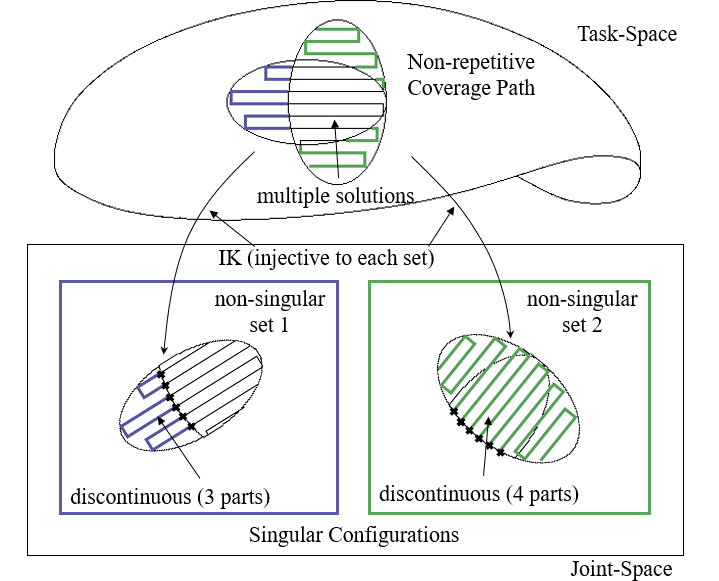
\includegraphics[width = 0.44\textwidth]{fig1}
\caption{A diagram showing the relation between the joint-space and the workspace. The non-singular configurations form disjoint sets which are denoted by different color. 
The colored parts of the path have unique IK solutions. 
However, for the path with black line, there are multiple IK solutions, which requires further decision. 
Besides, the continuous path in the workspace is no longer continuous after mapped into the joint-space. In this example, whatever choice among the multiple IK solutions, $8$ discontinuities are required, since the path has five separated parts in set $1$ and four parts in set $2$. 
}\label{fig1}
\end{figure}

People have noticed that the singularities are the cause of the bifurcation of the joint-space \cite{porta2010path} \cite{Porta2012Randomized}. In the coverage task, the singular configurations are useless because of the loss of manipulability. Thus, all non-singular configurations form disjoint sets in the joint-space. See Figure \ref{fig1} for illustration. 
What we further notice is that the IK mapping from the reachable points in the workspace to a single set of configurations is injective. 
The reason is that, the different IK solutions come from different solutions of the inverse trigonometric function, between which the joint angle goes through a singular angle. 
As a result, different IK solutions for a same pose belongs to different sets.
Due to the constraints, commonly the whole workspace cannot be mapped into a single set, then the continuous joint-space path must visit some singularities, inevitably causing lift-offs. 

There are many significant works looking for the optimal coverage paths \cite{Atkar2003Towards} \cite{huang2001optimal}, but the variation of the cost between different continuous coverage paths is far less than that of one extra discontinuity. Also, there are many literatures \cite{cheah2003brief} \cite{heck2015switched} \cite{mirrazavi2018a} \cite{solanes2018adaptive}, \cite{solanes2019robust} discussing reducing the cost during the contacting and maintaining smooth and stable transition, none of them notices that a coverage path without unnecessary lift-offs is solvable. 
\cite{paus2017a} considers optimizing the position of the mobile manipulator for coverage task, which strengthens the requirement of a valid criterion of the relative pose between the manipulator and the object. 




In this paper, we make the following contributions: 

(1) Prove that the least number of lift-offs for a non-repetitive coverage task using non-redundant manipulator is a parameter of the environment setting (the related pose between the manipulator, the object and all obstacles), independent to the choice of the physical coverage path. Hence it becomes a criterion evaluating the quality of the placement of the manipulator (or the object). 

(2) Propose a novel cellular decomposition method which divides the surface into least number of cells, ensuring that each cell can be covered without lift-off through the specified configurations. 


The remainder of this paper is organized as follows. Section \ref{sectionrelatedwork} reviews the existing literature. 
%Section \ref{sectionproblemformulation} presents a formal definition of the problem. Section \ref{sectionalgorithm} presents the structure of our algorithm. 
Section \ref{sectionproblemformulation} states the problem, models the problem into an abstract form that painting a graph using least number of colors and proves that the number of discontinuities is independent to the coverage path. 
Section \ref{sectionenumerativesolver} discusses the process of solving a single element. Section \ref{sectioniterativesolver} presents the iterative strategy to solve the whole problem. Section \ref{sectionexperiment} shows the experimental results, and Section \ref{sectionconclusion} concludes the paper. In the sequel, we use ``optimal path'' to represent a coverage path that requires least number of discontinuities, and present our algorithm in the language of the polishing task. 



\section{Related Work}\label{sectionrelatedwork}
The CPP problem is looking for a path that passes all points within a given area. 
Since it can be formulated into the Travelling Salesman Problem (TSP) \cite{choset2001coverage}\cite{galceran2013a}, which is thought as an NP problem, almost all state-of-the-art methods first decompose the given area and then solve the CPP problem in each cell. 

The CPP algorithms can be mainly divided into two categories: the exact cellular decomposition methods and the morse-based cellular decomposition methods. 
The exact cellcular decomposition methods \cite{lumelsky1990dynamic} divide the free space into several simple, easy sub-regions, and use conventional coverage paths, such as the trapezoidal path \cite{choset2005principles} or the boustrophedon path \cite{choset1998coverage}\cite{choset2000coverage}, to finish the coverage in each cell. 
The morse-based cellular decomposition methods apply the divisions of the free space based on the critical points of Morse functions \cite{choset2000exact}\cite{Acar2002Morse} to  present more flexible shape for cells than the exact cellular decomposition. 

The optimal CPP algorithms mainly focus on the path length and time to completion.
Atkar et al. presented a CPP algorithm for the spray painting robots \cite{Atkar2003Towards}. It maps the conventional coverage path to the 2.5D surface and optimizes the coverage path through choosing optimal starting point. 
Huang presented an optimal line-sweep based method for cellular decomposition algorithms in planar spaces \cite{huang2001optimal}. It covers each cell with sweeping path going in different directions to minimize the number of returns. However, this approach does not take into account the cost of traveling between cells. 
Jimenez proposed to use a genetic algorithm to achieve optimal coverage \cite{jimenez2007optimal}. The free space is divided into sub-regions using the trapezoidal cellular decomposition, then a genetic algorithm is used to plan an optimal path that covers all the subregions.  
Mannadiar and Rekleitis proposed an algorithm that achieves complete coverage of spaces while minimizing the path \cite{mannadiar2010optimal}. The algorithm encodes the cells to be covered as edges of the Reeb graph. Then, the optimal solution to the Chinese Postman Problem is used to calculate an Euler tour, which guarantees complete coverage and the minimum of path length. 

Searching for such a path with least number of discontinuities  for the manipulator is not trivial. However, none of the existing literatures paid attention to it. 
Since the mobile robots cannot leave the ground, it is impossible for a CPP algorithm designing for the mobile robots that considers this contact loss. As for the contact task of the manipulator, most of the literatures \cite{solanes2018adaptive} \cite{solanes2019robust} focus on the control strategies instead of avoiding detaching and re-touching the surface as many as possible. 



\section{Problem Formulation}\label{sectionproblemformulation}
In this section, we first state the optimal cellular decomposition problem of least number of discontinuites. Then, the equivalent problem that painting a graph into least number of pieces is created. Finally, we show that the least number of discontinuities is independent to the choice of the physical coverage path. 



\subsection{Problem Statement}

Given the surface of an object, the structure of the  manipulator, the shape of other obstacles and their relative poses, the required coverage path consists of all valid configurations which satisfy the following constraints:

(1) Kinematic Constraint: The manipulator is collision-free during the whole process. And when the EE contacts the surface, its $z$-axis is align with the normal vector of the surface at the contact point. 

(2) Force Constraint: When the EE contacts the surface, the manipulator should be able to exert the required force on the EE in the $z$-axis.  

(3) Manipulability Constraint: When the EE contacts the surface, the manipulator should keep well-conditioned (under some given  manipulability measure) to deal with the pertubation.

\noindent
One lift-off of the manipulator is denoted by a continuous piece of configurations in the path during which the EE does not contact the surface.
Then, the optimal cellular decomposition problem is to find a valid path of configurations which covers the workspace non-repetitively and ensures the minimum number of the lift-offs.
%\begin{color}{blue} 
In this problem, the contact area between EE and the surface is seen as a particle.
%\end{color} 

\begin{figure}[t]
\centering
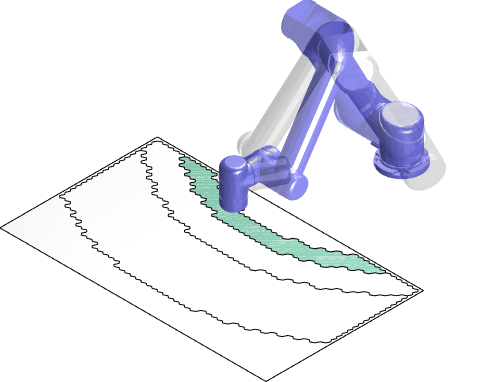
\includegraphics[width = 0.15\textwidth]{square_example/simple_example_merged_545}
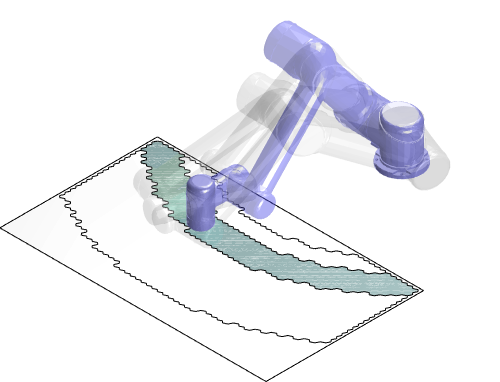
\includegraphics[width = 0.15\textwidth]{square_example/simple_example_merged_551}
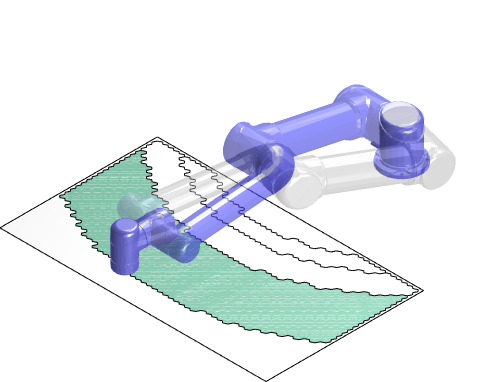
\includegraphics[width = 0.15\textwidth]{square_example/simple_example_merged_565}
\caption{The manipulator is polishing a planar rectangular object. The nearest and the farthest area are unreachable. Within the middle area, there are four kinds of configurations to polish the middle part, but only two of them can also polish the inner part and the outer part. Note that the vivid configurations in figures can be continuously reached (without lifting off the EE).}\label{figsquare}
\end{figure}

\begin{figure}[t]
\centering
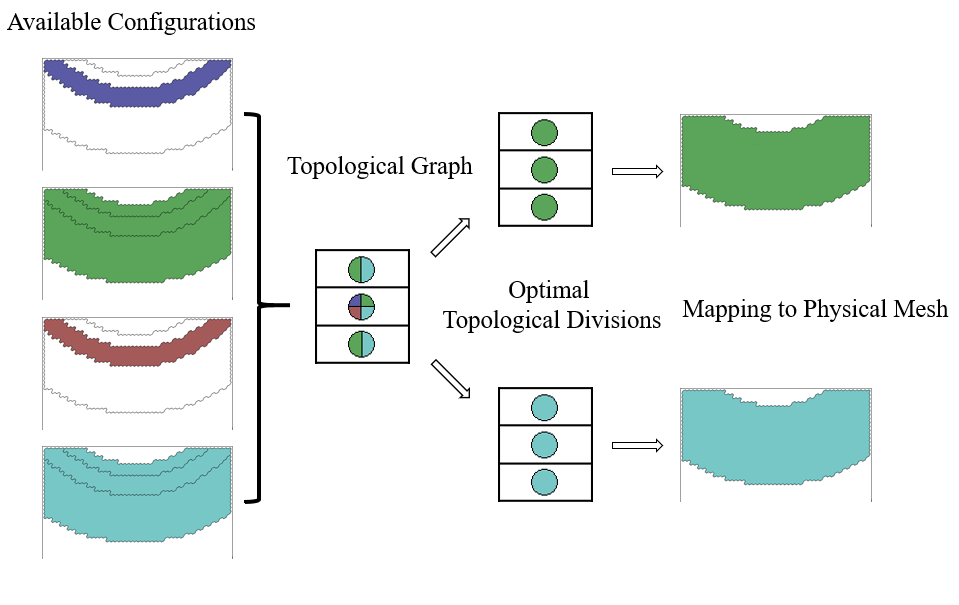
\includegraphics[width = 0.44\textwidth]{flowchart}
\caption{
Flowchart of our algorithm in solving the problem of Figure \ref{figsquare}. 
All configurations are divided into four disjoint sets, represented by different colors. 
The small circle filled in with color(s) shows all possible colors to paint the corresponding area. The topological graph is created based on the distribution of the colors and being solved. Finally, in this example, we can get two optimal options which both require zero lift-off. 
}\label{flowchart}
\end{figure}


\begin{figure}[t]
\centering
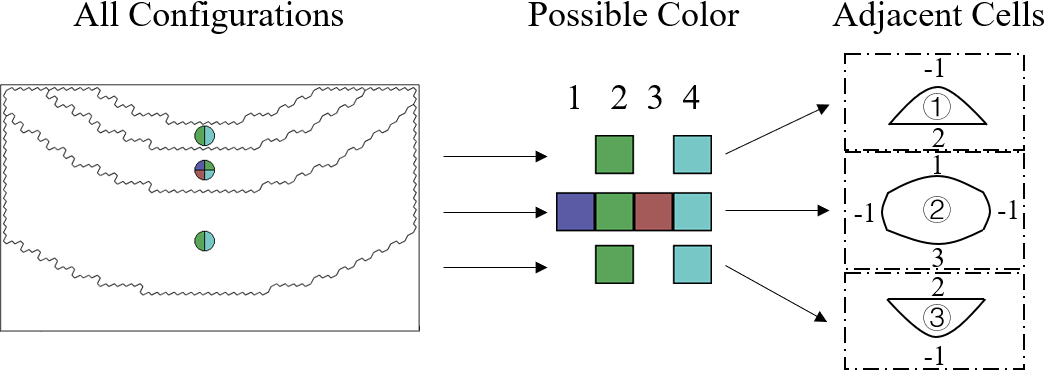
\includegraphics[width = 0.44\textwidth]{square_example/graphcreation}
\caption{The elements of a cell. All colors are indexed. Each cell corresponds to a connected area on the surface of the object and has a list of possible colors. The cell stores the index of its adjacet cell in order. The index of the unreachable area is denoted by $-1$. We use curves to show that the edge is topological but not physical. }\label{figforcolor}
\end{figure}



\subsection{Problem Modeling}\label{sectionmodelling}

Without loss of generality, the input data is a triangular mesh, with all vertices and edges fully known. Then the normal of each vertex and all valid IK solutions to cover it are also known. 
Since the manipulator is non-redundant, the number of IK solutions for each vertex is finite. 
Although the mesh is a discretized data structure, we say two vertices are ``continuous'', if there is a list of edges of the mesh connecting them. And we say two configurations are ``continuous'' for the manipulator to reach, if the vertices are continuous, and the distance of these two configurations in the joint-space is near enough. The distance threshold for the continuity is easy to judge, since the manipulability constraint abandones the configurations which are close to the singularities, thus creates an apparent gap between disjoint sets. Typically, just the signs of the joint angles are enough to judge the continuity of two configurations. For example, it is easy to see that three vivid configurations in Figure \ref{figsquare} are continuous, and the greyed out configurations in a same figure are discontinuous pairwise. 

First, we assign the color of all configurations. Starting from an unassigned configuration, using a floodfill-like algorithm on the mesh, all configurations which are continuous with the chosed one are easy to find and are assigned with a same number, which is the index of the corresponding color. After repeating the assignment process, all configurations have a color, and the continuous configurations have a same color. 
Note that the IK solutions for the same vertex must have different colors. 
So it is suitable to show the distribution of a color through drawing them on the mesh. For example, Figure \ref{flowchart} shows the distribution of four colors of the example in Figure \ref{figsquare}.
%So the colors of a vertex denotes all possible configurations to cover the vertex. 

Second, we divide the mesh into several ``cells'', with each vertex belonging to a cell. The cell is a connected open region containing all vertices which are continuous and can be covered through same kinds of colors. 
For the generation of a cell, we pick up an unassigned vertex, using a floodfill-like algorithm to find all continuous vertices which have same kinds of colors. 
These vertices belongs to a single cell. In Figure \ref{flowchart}, we draw a small circle filled in with multiple colors to show the possible colors for a cell. After repeating the process, all vertices are assigned. 

Third, after the creation of all cells, we say there is a topological edge between two cells, if there is a physical edge of the mesh which connects two vertices from different cells. 
We may see the intersection of topological edges in the following figures, but note that they are formally drawed, since each edge connects only two vertices which are impossible to belong to three or more different cells. 
In all, the structure of the topological graph is uniquely decided by the mesh. 

Finally, the cell records the possible colors for covering the points and the index of its adjacet cells in order, see Figure \ref{figforcolor}. 
%\begin{color}{blue}
%First we define some symbols. Let $\mathscr{C}$ be the set of all valid configurations (then no singularities in $\mathscr{C}$) and $\mathscr{C}_M$ be the set of all reachable points on the 2.5D surface. The pose of the EE is also denoted by $\mathscr{C}_M$ since there is an $1-1$ correspondence between the pose of the EE and the point on the surface, so we do not distinguish them. \\
%Since the manipulator is omni-directional in the joint space, given a configuration $p \in \mathscr{C}$ covering $p_M\in \mathscr{C}_M$, there exist a set of configurations $U_p\subset \mathscr{C}$ that can be reached without lifting the EE from $p$, covering a neighbourhood $U_{pM}\subset \mathscr{C}_M$. 
%(See Figure \ref{figsquare}, the poses of the manipulator in vivid color show three poses that can be reached continuously, so they belong to a same set. 
%If any of them is chosen as $p$, then all of them are in $U_p$. )
%If there are some other unassigned configurations, i.e., $\mathscr{C}\backslash U_p\neq \varnothing$, we choose another one $p'\in \mathscr{C}\backslash U_p$, then it specifies another set $U'_{pM}\subset \mathscr{C}_M$, and of course $U'_{pM} \cap U_{pM} = \varnothing$. 
%Without strict proof, after continuing this process for finite times, all configurations are assigned, then $\mathscr{C}$ is divided into several disjoint sets. 
%It is worth saying that the mapping between $U_p$ to $\mathscr{C}_M$ is an 1-to-1 mapping, since we cannot find a path in the joint-space connecting two inverse kinematic solutions of a same pose of EE without visiting a singularity. (i.e., in each figure of Figure \ref{figsquare}, the greyed out configurations have the same pose of the EE with the vivid one, so they do not belong to a same set. )
%Therefore, we can use the color on $U_{pM}$ to represent $U_p$. (For example, the visualization of different sets of $\mathscr{C}$ is shown in Figure \ref{flowchart}, and we know that $\mathscr{C}$ is divided into 4 disjoint sets.) The area with multiple colors means that there are multiple choices of valid configurations to continuously cover all points in this area. (For example, in Figure \ref{flowchart}, the middle part of the mesh can be covered by four colors, but the inner part and the outer part can only be covered by two colors).  
%Finally, we create the topological graph of the surface $M$, whose element is called ``cell'' where all points are connected and all have same kinds of possible colors. The cell records the possible colors for covering the points and the index of its adjacet cells in order, see Figure \ref{figforcolor}. 
Note that in practical application, since the area of the surface is finite, and each cell must have least size to keep the decomposition meaningful, the number of cells must be finite. 


After creating the topological graph, the original problem is equivalent to painting all points with one of their available colors, ensuring the minimum pieces of colors. And for a fully-filled graph, the color of a point uniquely specifies one of the valid IK solutions to cover it. 

\subsection{Independence from the physical coverage path}

%\begin{color}{blue}
%Since the manipulator is omni-directional in the joint space, each cell is 
%given a configuration $p \in \mathscr{C}$ covering $p_M\in \mathscr{C}_M$, there exist a set of configurations $U_p\subset \mathscr{C}$ that can be reached without lifting the EE from $p$, covering a neighbourhood $U_{pM}\subset \mathscr{C}_M$. 
%\end{color}
Since the manipulator is omni-directional in the joint-space, we can always find a continuous coverage path for a connected region in the joint-space. 
From the above definition of the cell, all points in a same cell have same kinds of colors, thus can be covered through some kinds of configurations which are represented by the colors, without lifting off the EE. 
Let the number of the cells be $n$, then if we design a coverage path within each cell, and directly concatenate these paths through paths with the EE leaving the surface, the total number of lift-offs is at most $n-1$. 
Since the number of cells is finite, the number of lift-offs is also finite. And because the creation of the initial graph depends only on the IK solutions of all points but not their order, the minimum number of lift-offs is a parameter of the environment setting and independent to the choice of the physical coverage path. 

\section{Enumerative Solver}\label{sectionenumerativesolver}
The difficulty of solving the coloring problem is that, although the points are gathered into a same cell, they can be filled in with different colors, 
instead of only being seen as a whole and drawn with a single color, see an easy example in Figure \ref{figsimpleexample}. 
We observe that the structure of the graph reflects in the connectivity of the topological edges, which is proved having only finite possible situations in \ref{subsectionproof}. 


\begin{figure}[t]
\centering
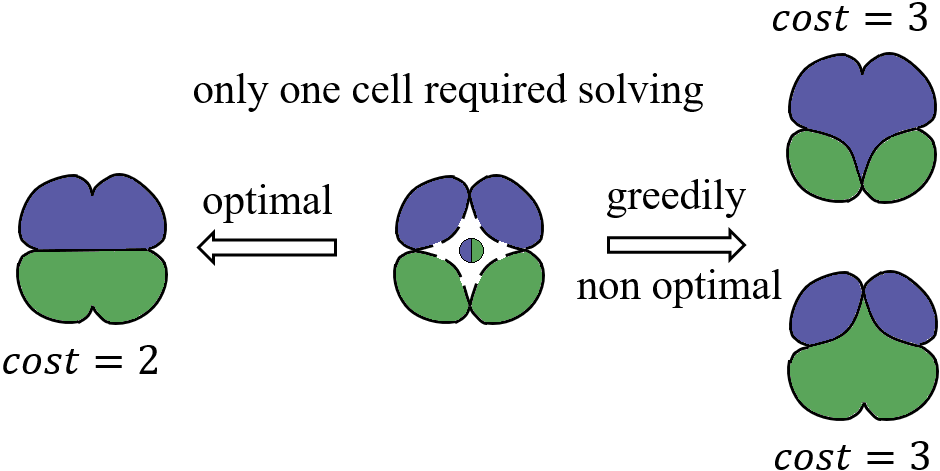
\includegraphics[width = 0.33\textwidth]{simple_example/simple}
\caption{In this graph, the boundary four cells only have one possible color and only the middle one needs solving. 
If the colors are chosed greedily, the middle cell must be filled in with pure color (like the right side), whose final cost will be $3$. However, if the middle cell is cutted into two parts, then two pairs of adjacent cells are connected and the cost will be $2$, which reaches the optimality. Note that the cutting path is arbitrary with the same function.}\label{figsimpleexample}
\end{figure}


In this section, we prove the finiteness of the number of divisions and introduce the enumerative solver through the example of solving a single cell with all its adjacent cells having been colored. We show that the simple cells with less than $4$ topological edges can be enumeratively solved, and there are finite number of manners to divide a complicated cell into several simple cells, hence any cell can be solved. 

\subsection{Finiteness of Divisions}\label{subsectionproof}
Since any path starting and ending at the boundary of a cell will divide the cell into two parts, there are infinite many physical solutions of dividing a cell into parts. However, there are only finite classes of them in the view of topological structure, because of the equivalence of physical divisions in the number of lift-offs. 

See Figure \ref{figproof}(a), we show that the cutting paths which start or end at an ordinary point on some edges are unnecessary. 
Let a cutting path ends at an ordinary point of the edge connecting cell 3. From the definition of a cutting path, it implicitly enforces cell 1 and cell 2 having different colors. Then we may assume $1=3$ or $2=3$ (when $1\neq 3$ and $2\neq 3$ the division is trivial), which, however, is equivalent to two other cutting paths that start at the endpoint of the edge. Do the same discussion on the other endpoint of this cutting path, we know that it is complete to only consider all cutting paths which start and end at the endpoint of some edges.  


See Figure \ref{figproof}(b), we show that the cutting paths which go across some edges are unnecessary. Let a cutting path go across the edge that connects cell 4. 
The cutting path can be continuously transformed onto the edge without changing the cost. 
This division enforces the constraint of color that $3\neq 4, 3\neq 5, 3\neq 6$. However, it prevents cell 5 and cell 6 from being colored together, because they are separated physically by the cell 3, which may increase the cost and is not optimal. So we can directly discard the cutting paths which go across edges. 

See Figure \ref{figproof}(c), we show that the cutting paths need not go across each other. When two cutting paths intersect, we can change the belonging of the path segment, and then the cutting paths can be continuously transformed onto the existed topological edges. So it is complete to discard the choices of cutting paths which have intersections. 


\begin{figure}[t]
\centering
\subfigure[The unnecessity of having a cutting path which starts or ends at an ordinary point of a topological edge. ]{
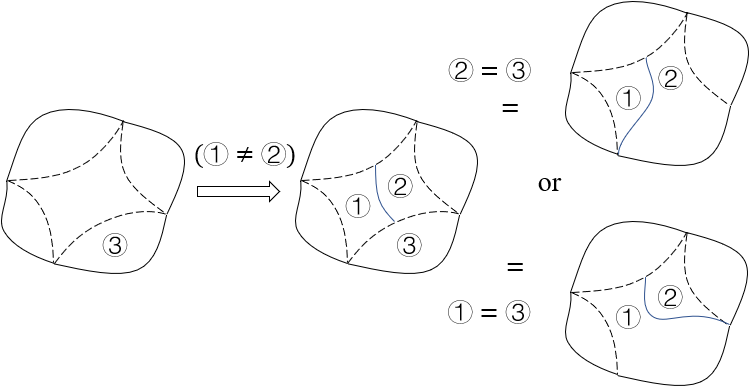
\includegraphics[width=0.4\textwidth]{proof/equiv_cutting_path}
}
\subfigure[The unnecessity of having a cutting path going across an edge. ]{
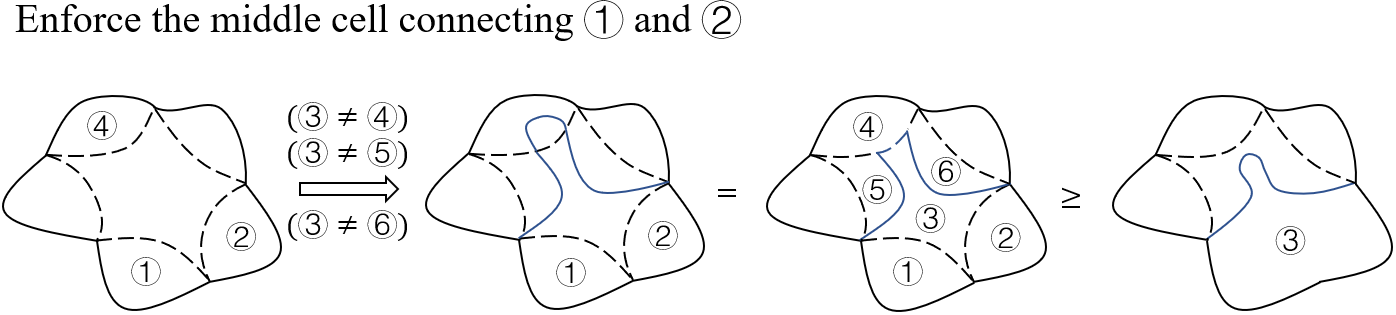
\includegraphics[width=0.48\textwidth]{proof/equiv_cutting_path2}
}
\subfigure[The unnecessity of intersecting two cutting paths.]{
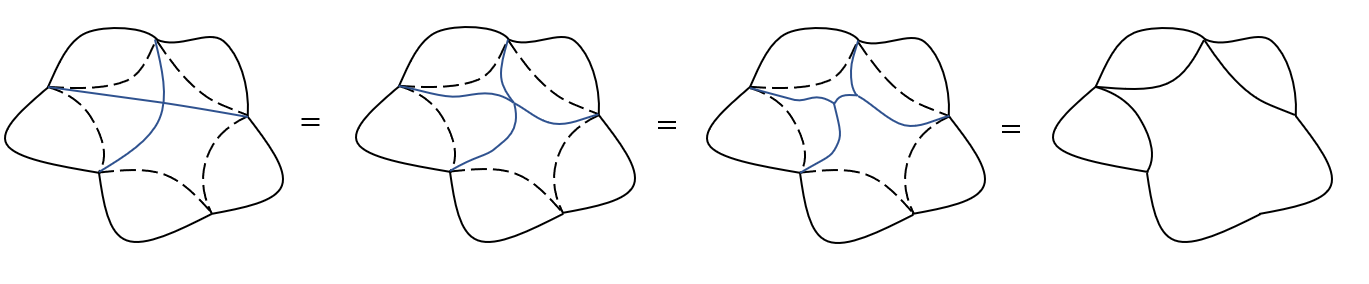
\includegraphics[width = 0.48\textwidth]{proof/equiv_cutting_path3}
}
\caption{Some physical divisions that are unnecessary or not optimal. }\label{figproof}
\end{figure}

In conclusion, we only need to consider all cutting paths which start and end at the endpoint of some topological edges and do not go across each other. Hence, the total number of topological divisions is finite and we just need to go through all possible divisions. 


\subsection{Solution of Simple Cells}
The following kinds of cells are so simple that can be solved directly without further divisions:

(1) The cells containing less than four edges,

(2) The cells with only one possible color,

\noindent
because the cells of (1) cannot be divided further into several cells with less number of topological edges, and the cells of (2) have no other choice of color. We enumerate all possible topological divisions of a 3-edge cell (which is the most complicated case for direct enumeration) in Figure \ref{figeasycell3}. We use a binary number to represent the connectivity of the edges, $1$ for connection, $0$ for disconnection. It is easy to see that there are at most $8$ situations.

\begin{figure}[t]
\centering
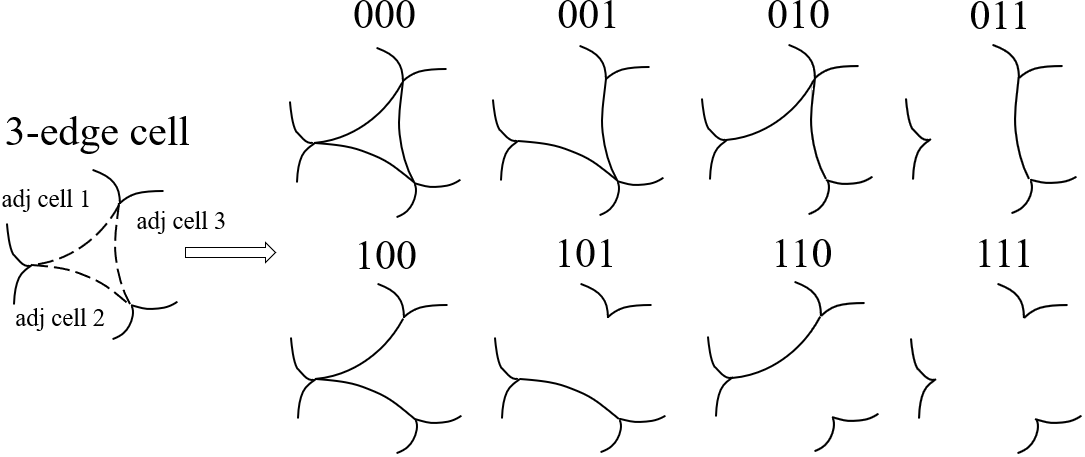
\includegraphics[width = 0.44\textwidth]{easycell/cell3}
\caption{All possible divisions of a 3-edge cell, which is the most complicated situation that need not further divisions. Although some of them are the same in the topological structure (e.g., $001, 010$ and $100$), or the division is impossible (e.g., we enforce $011$ but the cell 1 and cell 2 do not have a same color), it has already been a finite problem, so we omit the description of further simplification. }\label{figeasycell3}
\end{figure}


\subsection{Solution of Complicated Cells}


Following the idea of solving a simple cell, we use a binary number of length $n$ to represent the connectivity of an $n$-edge cell, $1$ for connection, $0$ for disconnection and $\times$ for the unspecified state. 
The continuous $1$s imply that part of this cell must be painted with the same color as that of which the $1$s specify. 
The $0$ means that the topological edge between the cell and the corresponding adjacent cell is keeped so that the colors must be different. 
The unspecified states $\times$ imply the generation of a sub-cell. An example of solving a 4-edge cell is shown in Figure \ref{figeasycell4}. Through specifying the position of $1$s, there are less than $2^n\times m$ branches for an $n$-edge cell with $m$ possible colors, so the problem is finite. The distinguishment between $0$ and $\times$ will be given in subsection \ref{subsectiondiscussion}.

\begin{figure}[t]
\centering
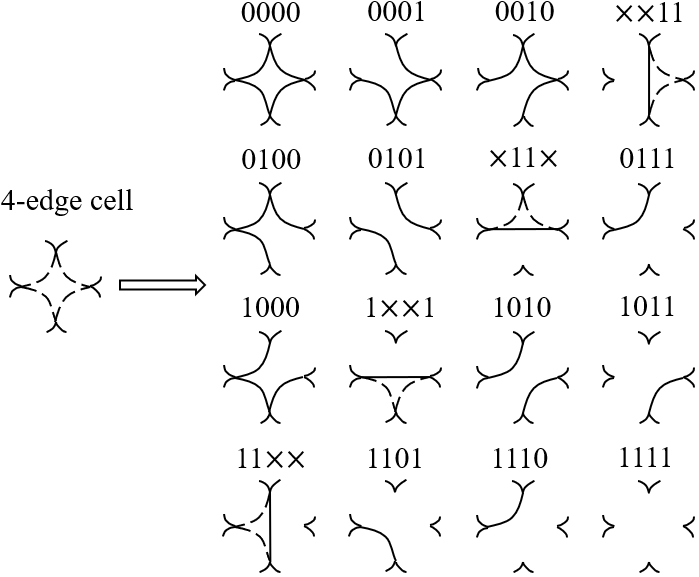
\includegraphics[width = 0.4\textwidth]{easycell/cell4}
\caption{The $2^4$ possible divisions of an 4-edge cell. For the cell which has more than 3 edges, the sub-cell may be created. In this figure, the connectivities that correspond to generating a sub-cell is $\times\times11, \times11\times, 1\times\times1, 11\times\times$. }\label{figeasycell4}
\end{figure}

\subsection{Discussion of Creating Sub-Cells}\label{subsectiondiscussion}
When there exist such number lists in the connectivities: 
$$1\times\times1, 1\times\times\times1, \cdots$$
the cell is divided into parts whose colors are enforced to be different, so called sub-cells.
See the case of $\times\times11, \times11\times, 1\times\times1, 11\times\times$ in Figure \ref{figeasycell4}. The original cell becomes a new one with fewer edges, becasue some edges are replaced by a single edge. We use the bracket $(\cdots)$ in the binary number of the original cell to represent the generation of sub-cells.
Do the same division for the sub-cells, any $n$-edge cell can be continuously divided into a set of 3-edge cells and then be solved enumeratively. 

Since the sub-cell is generated from an original one, there are extra constraints on its connectivity specified by the previous division. However, these constraints cannot change this problem into one with polynomial time solution, so we just give some examples among them:

(1) Single $\times$ cannot form a sub-cell, because 
$$\cdots 1\times 1\cdots = \cdots 101\cdots \mbox{ or }\cdots 111\cdots$$
but both conditions of the right side are considered in other branches. This is why there is no $\times$ in Figure \ref{figeasycell3}.  

(2) The $0$s can be freely moved outside the bracket, because of the equivalence 
$$\cdots\times1(0\times\cdots\times1)1\times\cdots = \cdots\times10(\times\cdots\times1)1\times\cdots$$
and the same is true for the right bracket based on the symmetry of the number list, because the cutting graph makes sense only when the inner boundary two numbers are $1$s. See Figure \ref{figconstraint}. This is why no brackets in Figure \ref{figeasycell4}.

(3) The new topological edge created by the cutting path must be keeped (always $0$, impossible to be $1$ or $\times$) because it is manually created. Hence, for the entire problem, no extra possiblities appear after the divisions 

\begin{figure}[t]
\centering
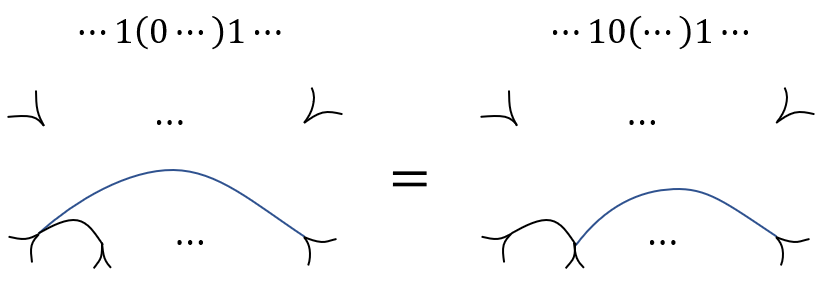
\includegraphics[width = 0.3\textwidth]{proof/equiv_zero}
\caption{The equivalence of moving the $0$ outside the bracket. In order to reduce the number of edges of the sub-cell, we always enforce the sub-cell looking like the right side. }\label{figconstraint}
\end{figure} 



\section{Iterative Solver}\label{sectioniterativesolver}

%\begin{color}{blue}
%The solving process is iteratively executed. In each iteration, the algorithm chooses an unsolved cell, finds its all possible solutions and creates a branch for each possible solution. In each branch, the chosed cell is filled in with the specified color (so it will not change any more). 
%Then, in the next iteration, the algorithm chooses an unsolved branch, chooses an unsolved cell in it and does the same steps as before. 
%Finally, after iteratively solving, each branch becomes a valid scheme for coloring or returns with a contradiction. 
%The algorithm runs like the deepest-first-searching (DFS) algorithm so that the memory requirement is not high. 
%\end{color}

\subsection{Iteration Process}
Regarding the enumerative solver as a basic step, we iteratively solve the graph. 
Starting from a fully-unpainted graph, we choose an unsolved cell and enumerativelly solve it. 
Assume that the cell has $n$-edges with $m$ possible colors, following our previous discussion, there are at most $2^n\times m$ possible divisions. We create a branch for each possible solution of the chosed cell, and in each branch the chosed cell is filled in with the specfied color (so it will not change any more). 
In the next iteration, we choose an unsolved branch, choose an unsolved cell in it and do the same steps as before. 
Note that the constraints given by the solved adjacent cells hugely restrict the possible solutions, because the state of an edge resticts the connectivity of the cells on both side. 
After iterative execution, all branches reach a contradiction or a valid coloring scheme. A valid coloring scheme for the graph uniquely specify the configuration to polish each point among its valid IK solutions. 
The algorithm runs like the deepest-first-searching (DFS) algorithm so that the memory requirement is not high. 
Since the execution is an exhaustive searching, all optimal physical cellular decompositions must be homeomorphic to one of our result schemes, with the position of the physical boundaries of the cells slightly different to the physical ones.

\subsection{Calculation of Cost}
The physical meaning of the cost for a (partly filled) graph is the number of pieces of color in the current graph. 
Describing the formula incrementally, after we solve a cell, 

(1) If its connectivity is all zero, then the cost will increase $1$ after coloring this cell, because this cell forms a new piece.

(2) If its connectivity has only one $1$ connecting a solved cell, then the cost will not change, because this cell can be filled together with the connected adjacent cell. 

(3) For its connectivity with $i$ $1$s, note that there may exist multiple edges which connect the same adjacent cell (See Figure \ref{figcost}). In order to be consistent with the physical meaning of the cost, if these edges connect $j$ distinct solved cells, then the variation of cost is 
$$\Delta cost = 1-j$$


\begin{figure}[t]
\centering
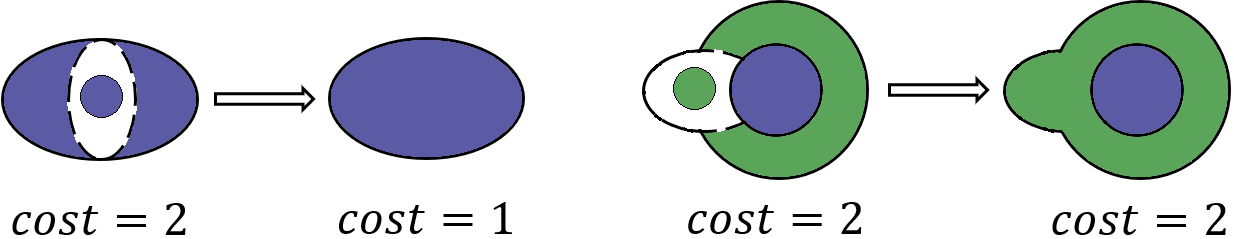
\includegraphics[width = 0.4\textwidth]{proof/costcal}
\caption{Left: the middle cell connects two distinct cells, so the cost variation is $1-2 = -1$. Right: two edges connect with the same adjacent cell, then the cost variation is $1-1 = 0$ but not $1-2 = -1$.}\label{figcost}
\end{figure}

\section{Experimental Results}\label{sectionexperiment}

Our algorithm works on any non-repetitive coverage task using non-redundant manipulators in any dimension. 
In this paper, experiments are taken by using a 5DOF manipulator to polish the surface of an object. And the manipulator should cover all reachable points even if it cannot fully cover the surface. 

Before showing the experiments, we state the calculation of the least number of lift-offs under other cellular decompositions, from which we can see that the proposed algorithm outperforms other methods. 
In the simulated experiments, we first show an object being polished at different poses, one casually and the other being designed precisely. We can see that the required number of lift-offs can distinguish them. Thus, the number can be seen as a criterion of the quality of the placement. Then, we show that our algorithm helps to get rid of bad configurations which result in extra lift-offs.
In the real-world experiment, the physical coverage path is set to see the proposed algorithm running in reality. 
\begin{color}{blue}
Through the attached video, we can see that the manipulator finishes the coverage task under minimum number of lift-offs. 
\end{color}

Unless otherwise stated, the environment contains only the manipulator, the object and the ground plane. 
For easy talking, the collision models of everything are the same as their visualizations. 
And note that all figures in this section are just an example of the optimal solutions. 
As we have discussed before, there are infinite many physical cutting paths of decomposition that result in same number of lift-offs of the EE, and the choices of the coverage paths within each cell are also arbitrary.


\subsection{Calculating least number of discontinuities for other methods}
In above sections we have talked the proposed algorithm running on a simply-connected surface. As a simple corollary, if the surface has been divided by other cellular decomposition methods, assumed into $n$ parts (where each cutting path implies a lift-off, then $n-1$ lift-offs are required), we can apply the proposed algorithm in each cell to know the least number of lift-offs required in each single cell, assumed as $p_i$ for the $i$-th cell. Finally, we will know that the least required number of lift-offs obeying the given cellular decomposition method is 
$$n-1 + \sum\limits_{i = 1}^n p_i$$ 
Obviously, applying the proposed algorithm to the cellular decomposition created by itself, the number $n$ is optimal guaranteed by the exhaustive searching, and each cell can be covered without lift-offs, which means $p_i = 0, \forall i$. Hence, the proposed algorithm certainly outperforms other methods in the sense of the number of lift-offs. 



\subsection{Covering a hemisphere}
In this experiment, through the polishing task of a semi-ellipsoid shape object, we show that the number of lift-offs provided by our algorithm can evaluate the quality of the placement of the object (or the manipulator). 

See Figure \ref{figflatwise}, a common scene is that, we place the object casually (flatly at $(0.7m, 0m, 0m)$ related to the manipulator) and start the CPP task, since there is no apparent criterion on the quality of the placement. However, the proposed algorithm shows that such a placement of the object requires at least $3$ lift-offs, but still fails in full coverage (the farthest area is unreachable), which is equivalent to at least $4$ lift-offs. 
Instead of the usual setting, see Figure \ref{figsloped}, if we precisely design the pose of the object (obliquely at $(0.7m, 0.1m, 0.08m)$), then not only the least number of lift-offs decreases to $2$, but the manipulator can fully cover the surface, which performs much better than the scene in Figure \ref{figflatwise}. Hence, the required number of lift-offs guides the user to try different poses of the object (or the manipulator) to have better performance on coverage. 


\begin{figure}[t]
\centering
\subfigure[]{
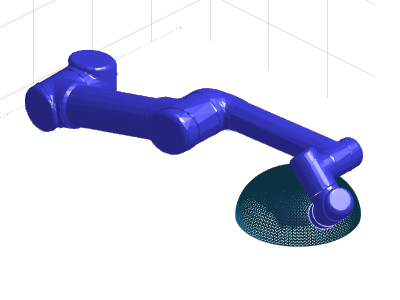
\includegraphics[width = 0.10\textwidth]{exp_semi_ellipsoid/casual_demo}
}
\subfigure[]{
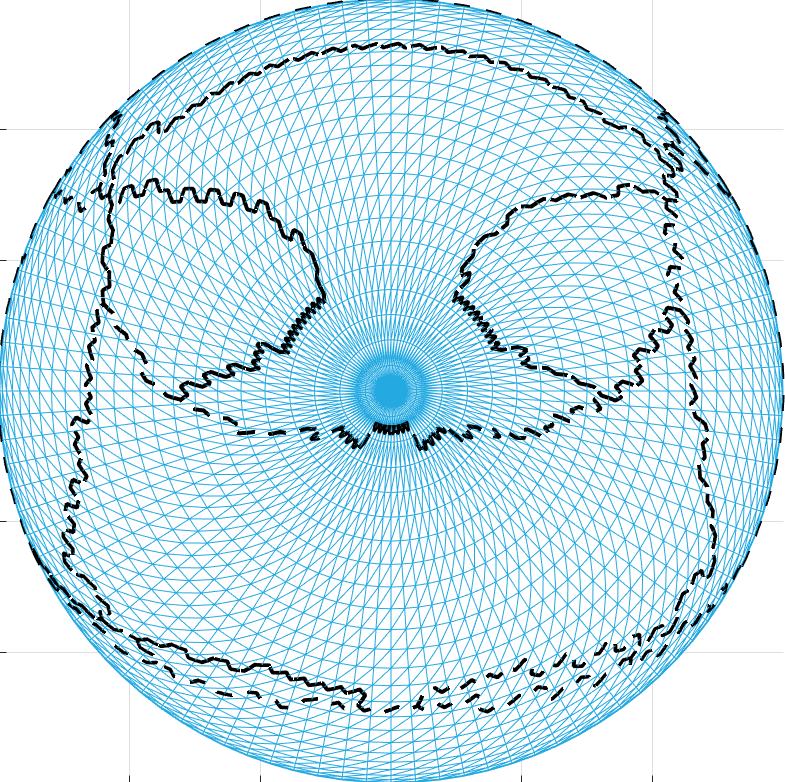
\includegraphics[width = 0.10\textwidth]{exp_semi_ellipsoid/casual_init_graph}
}
\subfigure[]{
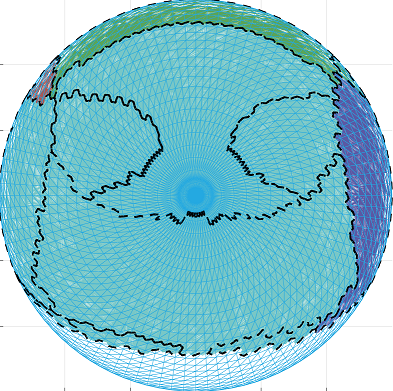
\includegraphics[width = 0.10\textwidth]{exp_semi_ellipsoid/casual_result_graph}
}
\subfigure[]{
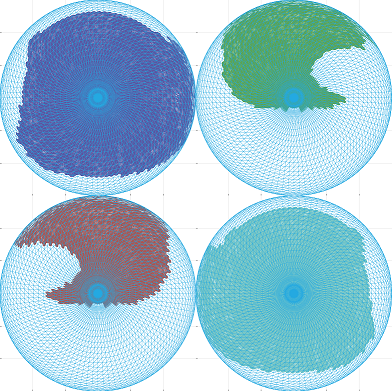
\includegraphics[width = 0.10\textwidth]{exp_semi_ellipsoid/casual_comb}
}
\caption{(a) The object is casually placed. (b) The initial graph. (c) One optimal solution which requires 3 lift-offs, but the manipulator still cannot fully cover the farthest part of the mesh (the top area in the figure). (d) The reachable area of four kinds of valid configuration chosed by the optimal solution in (c). 
}\label{figflatwise}
\end{figure}
\begin{figure}[t]
\centering
\subfigure[]{
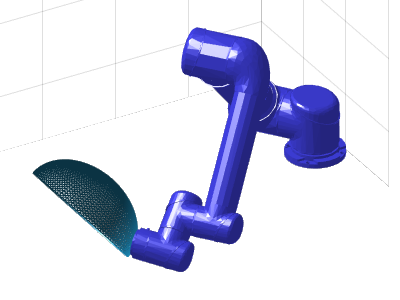
\includegraphics[width = 0.1\textwidth]{exp_semi_ellipsoid/design_demo}
}
\subfigure[]{
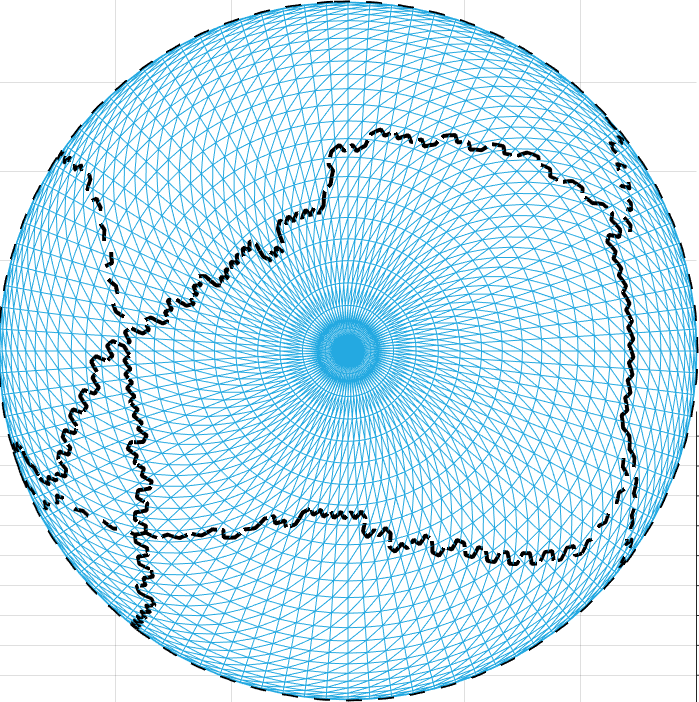
\includegraphics[width = 0.1\textwidth]{exp_semi_ellipsoid/design_init_graph}
}
\subfigure[]{
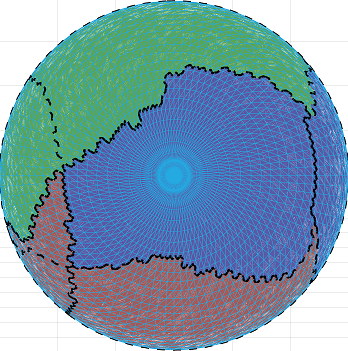
\includegraphics[width = 0.1\textwidth]{exp_semi_ellipsoid/design_result_graph}
}
\subfigure[]{
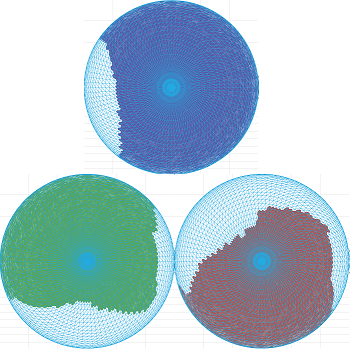
\includegraphics[width = 0.1\textwidth]{exp_semi_ellipsoid/design_comb}
}
\caption{(a) The object is placed obliquely. (b) The initial graph. (c) One optimal solution which only requires 2 lift-offs but realizes full coverage. (d) The reachable area of three kinds of valid configurations which are chosed by the optimal solution in (c). 
}\label{figsloped}
\end{figure}


\subsection{Covering a pipe}
In this subsection, through the polishing task of a half pipe, we show that the proposed algorithm can clearify the unnecessary configurations, avoid the ``trapped'' configurations which cause extra lift-offs. 

The pipe is placed obliquely (at $(0.45m, 0.45m, 0.45m)$ related to the manipulator). Althrough the object is common, the normal of its surface varies for $\pi$ rad, which causes difficulty for the manipulator. We show the initial graph and directly give its optimal solution in Figure \ref{fighalfpipe}. The optimal solution of this coverage task requires only $1$ lift-off. 

See Figure \ref{figthreeexamplepose} for an explaination of the distinguishability of the useless configurations. The first kind of configurations and the third one are finally chosed by the optimal solution. It is worth saying that, althrough the second kind of configurations can polish large area without lift-offs, which looks appealing and is very likely to be chosed if the IK solutions are chosed randomly, it cannot reach the corners of the mesh (which are eventually covered by the other two ones). If the manipulator uses any of the configurations belonging to the second kind, after the coverage of the main part, sooner or later it has to waste two lift-offs to finish the full coverage, which leads to non-optimality. 
\begin{figure}[t]
\centering
\subfigure[]{
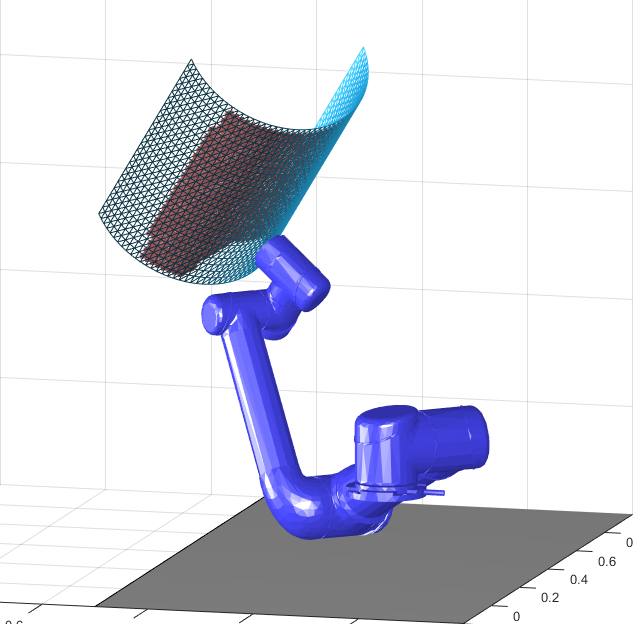
\includegraphics[width = 0.14\textwidth]{exp_pipe/demo}
}
\subfigure[]{
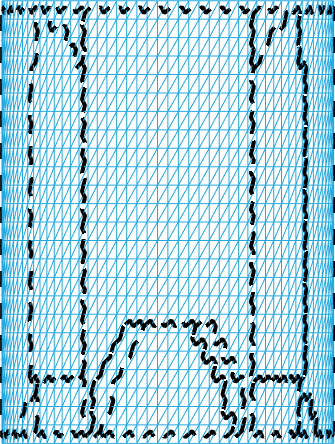
\includegraphics[width = 0.14\textwidth]{exp_pipe/init_graph}
}
\subfigure[]{
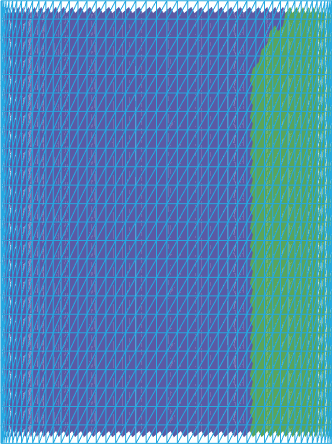
\includegraphics[width = 0.14\textwidth]{exp_pipe/result_graph}
}
\caption{(a) The manipulator is polishing the top-right corner where can only be polished through kinds of configurations. (b) The initial topological graph of this problem. (c) One optimal solution which requires 1 lift-off.}\label{fighalfpipe}
\end{figure}

\begin{figure}[htb]
\centering
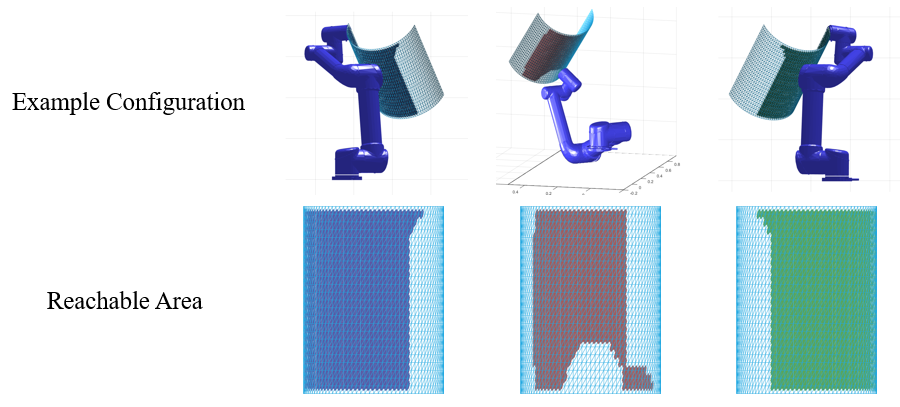
\includegraphics[width = 0.35\textwidth]{exp_pipe/three_example_pose}
\caption{Left: Example of three different kinds of configurations polishing a same point. Right: The coverage region for each kind of configurations. 
We omit the visualization of other kinds of configurations. Since  there is only one color to cover the top corners (the first one for the top-left corner and the third one for the top-right corner), once any configuration belonging to the second kind is mistakenly chosed to cover any area of the surface, sooner or later we have to change to the first one and the third one to finish the full coverage of the surface, which wastes an unnecessary lift-off.}\label{figthreeexamplepose}
\end{figure}

\subsection{Real World Experiments with Presence of Obstacles}

In this subsection, we use a manipulator polishing the outer surface of a wok to show a physical coverage path generated based on the proposed cellular decomposition method. 
The physical coverage path uses simple back and force motions, whose generation is not part of our concern. The concatenation between paths in different cells are created by demonstration. 
The manipulator is UR5, with its last joint abandoned, equivalent to 5DOF, which is non-redundant. 
Since the hybrid position/force control is beyond our contribution, we do not envolve the real contact. 

See Figure \ref{fig_realworld_no}, the nearest and farthest part of the wok are unreachable. 
Considering the two points shown in Figure \ref{fig_realworld_no}(d)(e), the manipulator has to keep its wrist ``above'' its fore-arm in order to avoid collision between them, which leads to the requirement of both shoulder-left configurations and shoulder-right configurations. 
The total number of lift-off is $1$. Since each color covers some points which only have one possible color, the solution is definitely optimal. Note that any division keeping the connectivity is optimal, so we may just divide the surface through the middle. 

See Figure \ref{fig_realworld_with}, the manipulator is obstructed by a cylindrical obstacle. Since the obstacle may collide with the upper-arm, fore-arm or the EE, and the wrist may collide with the fore-arm, to avoid all collisions, the least number of lift-offs is 2. Similarly, each color covers some points which only have one possible color, so the solution is also optimal. 

\begin{figure}[t]
\centering
\subfigure[]{
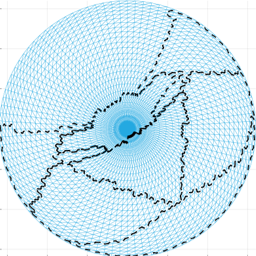
\includegraphics[width = 0.14\textwidth]{real_world_exp/no_obstacle_initial_graph}
}
\subfigure[]{
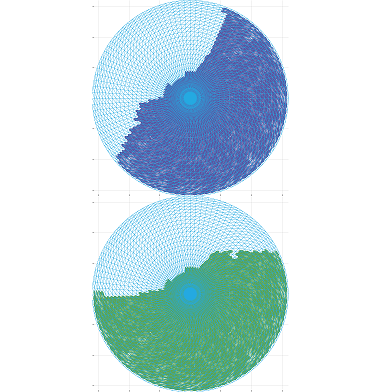
\includegraphics[width = 0.14\textwidth]{real_world_exp/no_obstacle_comb}
}
\subfigure[]{
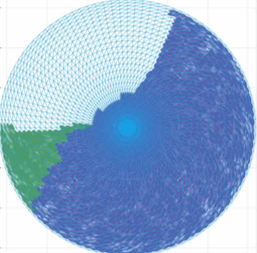
\includegraphics[width = 0.14\textwidth]{real_world_exp/no_obstacle_result_graph}
}
\subfigure[]{
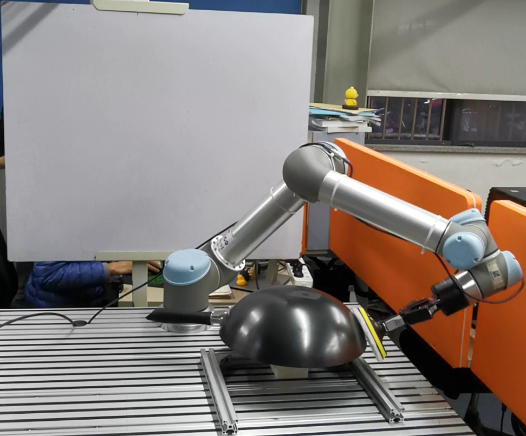
\includegraphics[width = 0.2\textwidth]{real_world_exp/no_obstacle_demo_1}
}
\subfigure[]{
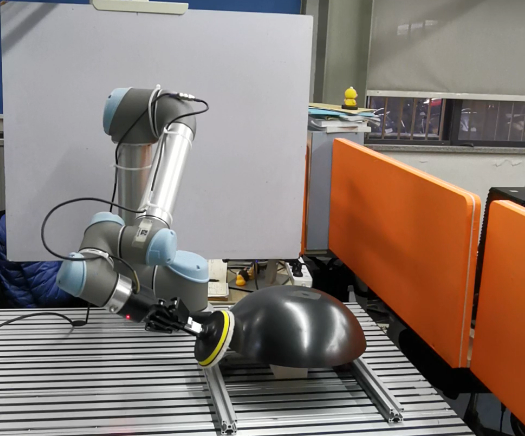
\includegraphics[width = 0.2\textwidth]{real_world_exp/no_obstacle_demo_2}
}
\caption{(a) Initial graph. (b) The reachable area of two kinds of configurations which are chosed by the solution in (c). (c) The cutting graph is arbitrary, so we may divide the graph through the middle. (d)(e) Example of the extreme poses of the two kinds of configurations. }\label{fig_realworld_no}
\end{figure}

\begin{figure}[t]
\centering
\subfigure[]{
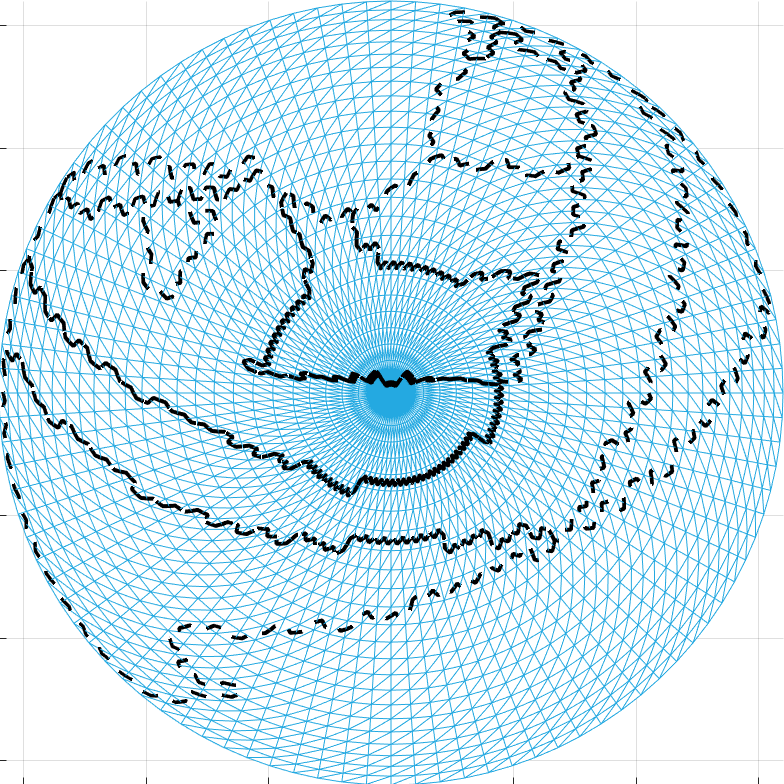
\includegraphics[width = 0.14\textwidth]{real_world_exp/with_obstacle_initial_graph}
}
\subfigure[]{
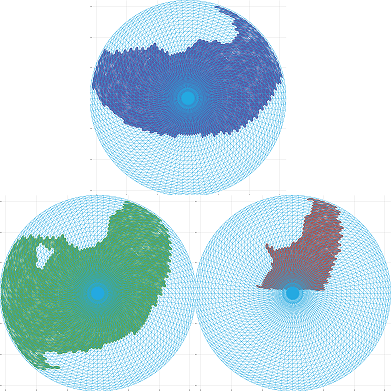
\includegraphics[width = 0.14\textwidth]{real_world_exp/with_obstacle_comb}
}
\subfigure[]{
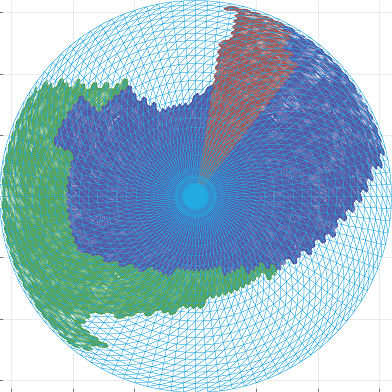
\includegraphics[width = 0.14\textwidth]{real_world_exp/with_obstacle_result_graph}
}
\subfigure[]{
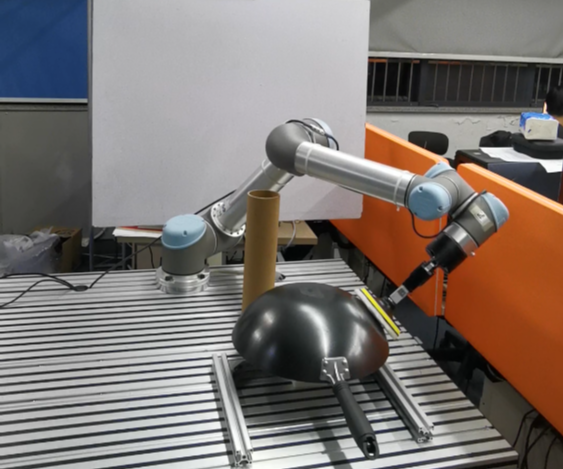
\includegraphics[width = 0.14\textwidth]{real_world_exp/with_obstacle_demo_1}
}
\subfigure[]{
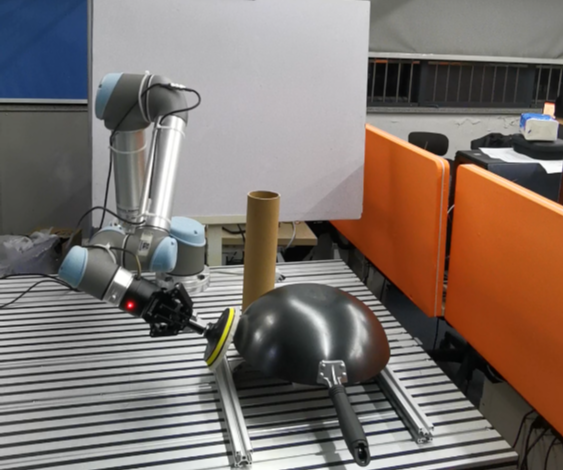
\includegraphics[width = 0.14\textwidth]{real_world_exp/with_obstacle_demo_2}
}
\subfigure[]{
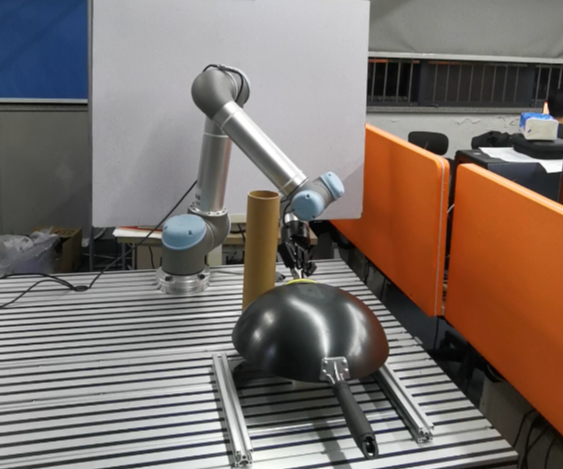
\includegraphics[width = 0.14\textwidth]{real_world_exp/with_obstacle_demo_3}
}
\caption{(a) The initial graph. (b) The reachable area of three kinds of configurations which are chosed by the solution in (c). (c) One optimal solution. (d)(e)(f) Example of the three kinds of configurations, where
(d) The shoulder-left configurations avoid collision between the upper-arm and the obstacle. (e) The wrist is above the fore-arm so that the wrist will not hit the fore-arm. (f) The only valid configuration to cover this point is putting the wrist below the fore-arm. }\label{fig_realworld_with}
\end{figure}

\section{Conclusion}\label{sectionconclusion}
In this paper, we first prove that the least number of the discontinuities is independent to the choice of the coverage path, thus becomes a criterion evaluating the quality of the placement of the manipulator (or the object), which may contribute to the mobile manipulator or the designing of the assembly line. Then, the proposed algorithm provides a novel cellular decomposition strategy, which, after applying the conventional CPP algorithm in each cell, generates the result coverage path containing the least number of discontinuities, which is verified through simulated and real-world experiments. 
Also, as a direct corollary, applied to the result of other cellular decomposition methods, the proposed algorithm can tell the user the least number of discontinuities obeying the given cellular decomposition. 

Because of the transition strategy which is more complicated than usual movement for coverage required by the discontinuities, and due to the unreachabiliy of the optimal coverage path, an NP problem, the optimality criterion of the coverage path that ensuring least number of discontinuities becomes more significant, and reducing the number of discontinuities is practical to reduce the cost of the coverage task, which is solvable through the proposed algorithm. 

In the future, a more complicated situation will be considered, where the initial topological graph contains ring-like cells, which can be broken during the iterative solving process. And the real contact process will be envolved to quantize the energy saving.









% An example of a floating figure using the graphicx package.
% Note that \label must occur AFTER (or within) \caption.
% For figures, \caption should occur after the \includegraphics.
% Note that IEEEtran v1.7 and later has special internal code that
% is designed to preserve the operation of \label within \caption
% even when the captionsoff option is in effect. However, because
% of issues like this, it may be the safest practice to put all your
% \label just after \caption rather than within \caption{}.
%
% Reminder: the "draftcls" or "draftclsnofoot", not "draft", class
% option should be used if it is desired that the figures are to be
% displayed while in draft mode.
%
%\begin{figure}[!t]
%\centering
%\includegraphics[width=2.5in]{myfigure}
% where an .eps filename suffix will be assumed under latex, 
% and a .pdf suffix will be assumed for pdflatex; or what has been declared
% via \DeclareGraphicsExtensions.
%\caption{Simulation results for the network.}
%\label{fig_sim}
%\end{figure}

% Note that the IEEE typically puts floats only at the top, even when this
% results in a large percentage of a column being occupied by floats.


% An example of a double column floating figure using two subfigures.
% (The subfig.sty package must be loaded for this to work.)
% The subfigure \label commands are set within each subfloat command,
% and the \label for the overall figure must come after \caption.
% \hfil is used as a separator to get equal spacing.
% Watch out that the combined width of all the subfigures on a 
% line do not exceed the text width or a line break will occur.
%
%\begin{figure*}[!t]
%\centering
%\subfloat[Case I]{\includegraphics[width=2.5in]{box}%
%\label{fig_first_case}}
%\hfil
%\subfloat[Case II]{\includegraphics[width=2.5in]{box}%
%\label{fig_second_case}}
%\caption{Simulation results for the network.}
%\label{fig_sim}
%\end{figure*}
%
% Note that often IEEE papers with subfigures do not employ subfigure
% captions (using the optional argument to \subfloat[]), but instead will
% reference/describe all of them (a), (b), etc., within the main caption.
% Be aware that for subfig.sty to generate the (a), (b), etc., subfigure
% labels, the optional argument to \subfloat must be present. If a
% subcaption is not desired, just leave its contents blank,
% e.g., \subfloat[].


% An example of a floating table. Note that, for IEEE style tables, the
% \caption command should come BEFORE the table and, given that table
% captions serve much like titles, are usually capitalized except for words
% such as a, an, and, as, at, but, by, for, in, nor, of, on, or, the, to
% and up, which are usually not capitalized unless they are the first or
% last word of the caption. Table text will default to \footnotesize as
% the IEEE normally uses this smaller font for tables.
% The \label must come after \caption as always.
%
%\begin{table}[!t]
%% increase table row spacing, adjust to taste
%\renewcommand{\arraystretch}{1.3}
% if using array.sty, it might be a good idea to tweak the value of
% \extrarowheight as needed to properly center the text within the cells
%\caption{An Example of a Table}
%\label{table_example}
%\centering
%% Some packages, such as MDW tools, offer better commands for making tables
%% than the plain LaTeX2e tabular which is used here.
%\begin{tabular}{|c||c|}
%\hline
%One & Two\\
%\hline
%Three & Four\\
%\hline
%\end{tabular}
%\end{table}


% Note that the IEEE does not put floats in the very first column
% - or typically anywhere on the first page for that matter. Also,
% in-text middle ("here") positioning is typically not used, but it
% is allowed and encouraged for Computer Society conferences (but
% not Computer Society journals). Most IEEE journals/conferences use
% top floats exclusively. 
% Note that, LaTeX2e, unlike IEEE journals/conferences, places
% footnotes above bottom floats. This can be corrected via the
% \fnbelowfloat command of the stfloats package.









% if have a single appendix:
%\appendix[Proof of the Zonklar Equations]
% or
%\appendix  % for no appendix heading
% do not use \section anymore after \appendix, only \section*
% is possibly needed

% use appendices with more than one appendix
% then use \section to start each appendix
% you must declare a \section before using any
% \subsection or using \label (\appendices by itself
% starts a section numbered zero.)
%


%\appendices
%\section{Proof of the First Zonklar Equation}
%Appendix one text goes here.
%
%% you can choose not to have a title for an appendix
%% if you want by leaving the argument blank
%\section{}
%Appendix two text goes here.


% use section* for acknowledgment
\section*{Acknowledgment}


The authors would like to thank...

\bibliographystyle{ieeetr} %% setting the cite style
\bibliography{min_removal}

% Can use something like this to put references on a page
% by themselves when using endfloat and the captionsoff option.
\ifCLASSOPTIONcaptionsoff
  \newpage
\fi



% trigger a \newpage just before the given reference
% number - used to balance the columns on the last page
% adjust value as needed - may need to be readjusted if
% the document is modified later
%\IEEEtriggeratref{8}
% The "triggered" command can be changed if desired:
%\IEEEtriggercmd{\enlargethispage{-5in}}

% references section

% can use a bibliography generated by BibTeX as a .bbl file
% BibTeX documentation can be easily obtained at:
% http://mirror.ctan.org/biblio/bibtex/contrib/doc/
% The IEEEtran BibTeX style support page is at:
% http://www.michaelshell.org/tex/ieeetran/bibtex/
%\bibliographystyle{IEEEtran}
% argument is your BibTeX string definitions and bibliography database(s)
%\bibliography{IEEEabrv,../bib/paper}
%
% <OR> manually copy in the resultant .bbl file
% set second argument of \begin to the number of references
% (used to reserve space for the reference number labels box)
%\begin{thebibliography}{1}
%
%\bibitem{IEEEhowto:kopka}
%H.~Kopka and P.~W. Daly, \emph{A Guide to \LaTeX}, 3rd~ed.\hskip 1em plus
%  0.5em minus 0.4em\relax Harlow, England: Addison-Wesley, 1999.
%
%\end{thebibliography}

% biography section
% 
% If you have an EPS/PDF photo (graphicx package needed) extra braces are
% needed around the contents of the optional argument to biography to prevent
% the LaTeX parser from getting confused when it sees the complicated
% \includegraphics command within an optional argument. (You could create
% your own custom macro containing the \includegraphics command to make things
% simpler here.)
%\begin{IEEEbiography}[{\includegraphics[width=1in,height=1.25in,clip,keepaspectratio]{mshell}}]{Michael Shell}
% or if you just want to reserve a space for a photo:

\begin{IEEEbiography}{Michael Shell}
Biography text here.
\end{IEEEbiography}

% if you will not have a photo at all:
\begin{IEEEbiographynophoto}{John Doe}
Biography text here.
\end{IEEEbiographynophoto}

% insert where needed to balance the two columns on the last page with
% biographies
%\newpage

\begin{IEEEbiographynophoto}{Jane Doe}
Biography text here.
\end{IEEEbiographynophoto}

% You can push biographies down or up by placing
% a \vfill before or after them. The appropriate
% use of \vfill depends on what kind of text is
% on the last page and whether or not the columns
% are being equalized.

%\vfill

% Can be used to pull up biographies so that the bottom of the last one
% is flush with the other column.
%\enlargethispage{-5in}



% that's all folks
\end{document}


